\documentclass[11pt]{book}

\usepackage[width=7.0in, height=9.0in, top=1.0in, papersize={8.5in,11in}]{geometry}
\usepackage[pdftex]{graphicx}
%\usepackage{datetime}
\usepackage{anyfontsize}
\usepackage{t1enc}
\usepackage{verbatim}
\usepackage{algorithm}
\usepackage{algorithmic}
\usepackage{framed}
\usepackage{pdfpages}
\usepackage{listings}
\lstset{language=C}

\lstset{language=python,frame=ltrb,framesep=5pt,basicstyle=\normalsize,
 keywordstyle=\ttfamily\color{DarkRed},
%morecomment=[n][\textbf]{In\ [}{]\:},
%morecomment=[n][\textbf]{Out\ [}{]\:},
morecomment=[s][\color{blue}]{In\ [}{]\:},
morecomment=[s][\color{red}]{Out[}{]\:},
identifierstyle=\ttfamily\color{DarkBlue}\bfseries,
commentstyle=\color{DarkGreen},
stringstyle=\ttfamily,
showstringspaces=false,tabsize = 3}


\lstdefinelanguage{shell} {
commentstyle = \color{black},
keywordstyle = \color{black},
stringstyle = \color{black},
identifierstyle = \color{black},
morecomment=[s][\color{blue}]{In\ [}{]\:},
morecomment=[s][\color{red}]{Out[}{]\:},
 }

\pagestyle{empty}

\usepackage{helvet}
\renewcommand{\familydefault}{\sfdefault}

\begin{document}

\fontsize{16}{16}\selectfont Sprint Report \#5


\section{Team Members:}
Marcus Berger
\\Dicheng Wu\\
\textbf{Sponsor:}
\\Jeff McGough
\\

\section{Prototype Progress}


Sprint five was dedicated to finishing the last of the functions and clean up of the project. First the client modified  some requirements for the team. After this the user stories remaining from sprint four were tackled by the group to produce the remaining payroll and billing interface. This included logging hours, and payments. After this was done the team started on bug fixes and quality of life updates such as new buttons and removal functions. The team is currently working on finishing up the student registration, and tax calculation for wages. If progress continues at this rate the prototype should be completed functionally however without some work the prototype may not reach some of the teams desired standard.


\section{Project deliverables of Sprint 5:}

Sprint 5 deliverables were the remaining functionality for the project. If the sprint was successful the main project will be done or very close to done functionally at the end of the sprint.


\subsection{Sprint 5 Backlog}

\begin{enumerate}
\item Admin and teacher update crossover
\item Ignoring case in address forms
\item Add rejected students to approved/ reject and provide current status
\item Multiple pay rates
\item Admin list function
\item Enter staff hours
\item Sprint 4 rollover (remaining payroll functions)
\item Add and remove class location
\item Removal Functions (Admin, Class, Student, Teacher)
\item Refunds and check boxes for fees and tuition
\item Quality of life updates to some functions
\item Bug Fixes
\item Student registration
\item Employee wages
\item Begin User Guide for documentation
\end{enumerate}


\section{Sprint 5}
During sprint five the team tackled the remaining functionally, bugs, and quality updates in an attempt to finish the base project. Removal functions to clean out the database were added, and some client requested quality of life updates were added. Bugs and glitches were patch up in many functions. Another job of this sprint was to finish the rollover from sprint four since some payroll functions still needed work. Lastly the team tackled student registration since the student interface was dropped from the project requirements in sprint 4. The registration is still in progress at this time, as the team failed to complete this functionality in time for the end of the sprint.

\section{Prorated Refunds}
The prorated refunds code will keep track of how much a class costed a student. If the student drops a class it will refund the remaining worth of the class to the students school credit field. This file has now been completed.

\section{Enter Staff Hours}
This page needed to undergo changes after meeting with client. The new version will allow a teacher to log their in class hours, office hours, trip hours, etc. These hours will then be paid out at their different rates respectfully. The hours will be logged as single numbers not by days or weeks. This function is now completed

\section{Enter Teacher Wages}
This was handled in the database in previous sprints assuming one pay rate. However in talks with the client the academy pays different pay rates based on what part of academy work they are doing. So the page will need to be updated once the list of possible pay rates have been provided by the client. This pages and its updates are still in progress. 

\section{Enter Tuition Rates and Fees}
Updated these pages to provide quality of life updates to the function requested by the client.

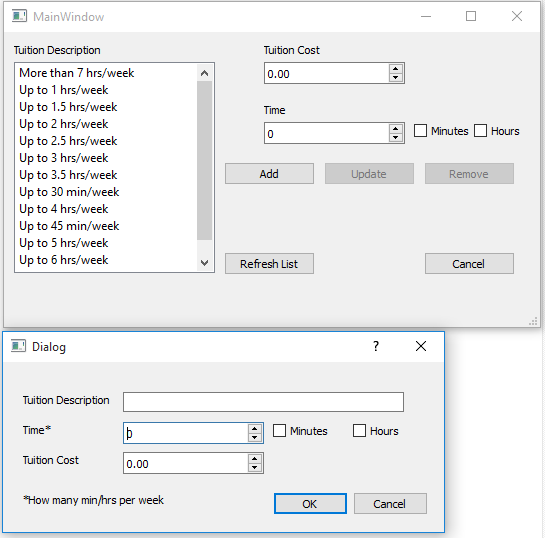
\includegraphics[scale=0.5]{tuitionRates.png}

\section{Bug Fixes}
During the coures of testing and the client meeting some bugs or inconsistences were discovered within the project. The bugs found and fixed are:

\begin{enumerate}
\item Student search was not showing all the students. Status: Fixed
\item Search edit need to be turned off and advance search modifications. Status: Fixed
\item Search, role, and schdules need to have dynamic not static times. Status: Fixed
\item Allow for time changes on schdule. Status: Fixed
\item Some of the back buttons in the teacher interface did not work correctly. Status: Fixed
\item Forms seem to be bugged at times, however can not recreate bug. Status: In testing possibly fixed.  
\end{enumerate}

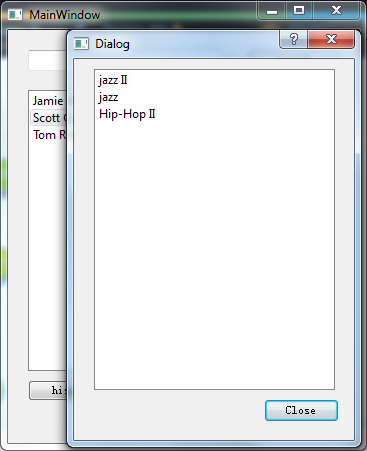
\includegraphics[scale=0.5]{teacherHistory.png}

\section{Updates Crossover}
One of the updates that needed to be completed this sprint was the need for admin and teacher updates to crossover if something was changed. This means that if someone is an admin and they update there phone number through the "update my information form" then the phone number will be updated in both the teacher table and the admin table. This way the system will not have conflicting information in different places. 

\section{Approved/Rejected Student Updates}
A update requested by the client was the ability to see rejected students in the approved/rejected pages just in case the academy changed its mind about a student. The page underwent slight modifications to the way information was displayed to make this change efficiently\\

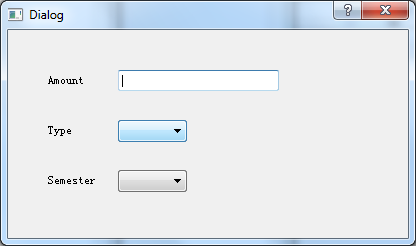
\includegraphics[scale=0.5]{payment.png}

\section{Admin List}
In creating some of the updates it became clear that a specific admin list was needed to see who had admin access to the system. This was done through a simple list view of the names that can then be selected to display more detailed information.\\
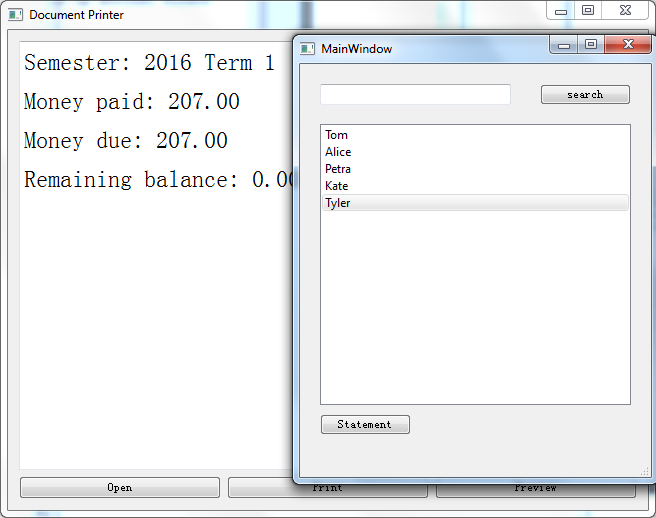
\includegraphics[scale=0.5]{invoice.png}

\section{Add/Remove Locations}
Another requested feature was the ability to add and remove locations for classes in the database. This feature is necessary because the academy sometimes teaches classes in different places based on need. The team accomplished this using a simple dialog that connects to the location table in the database. When the user updates or adds a new class the location combo box provides a list of locations in the database and an add location option.\\

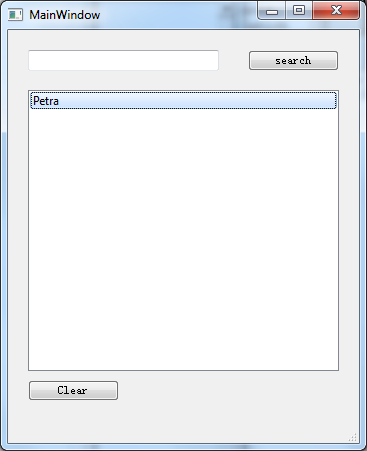
\includegraphics[scale=0.5]{enterPayment.png}


\section{Removal Functions}
These are simple functions that pull up a dialog box where the user can select a name and remove all the information related to that user from the system. The removal functions that exist in the system are: teacher, admin, student, and class. Teacher will remove that persons information from the system. Admin removes that persons admin rights and then ask if the whole user should be removed.


\section{Sprint 5 Issues}
Some issues that were encountered during this sprint were:

\begin{enumerate}
\item Spring semester ramp up - This was by far the biggest issue this sprint and the main cause of the failures this sprint. Other classes  up to the point of blocking work on many projects. Staggered due dates meant that when the team wanted to work, there was always another projects that needed to be completed in a short amount of time. By the end much of our time had been taken and the sprint began to fall behind.  
\item Requirement redefining - Due to drop the student interface the functionally needs to be added to the GUI which created some extra work for the team. 
\item Failure to complete backlog - The team did not finish all of the assign backlog this sprint.
\end{enumerate}

\section{Client Interactions}

Client interactions came in the form of required reviews and a demo of the prototype at the end of the sprint. Topics included:

\begin{enumerate}
\item Progress reports on where we are in the project
\item Asking questions to refine functionality, understand academy needs, and update requirements.
\item Discuss the future of the project and idea on how to execute them.
\item Prototype the current version of the prototype.
\end{enumerate}


\section{Group Meeting}

The group has a standard meeting time of TTH 10:00 - 12:00 and once during the weekend and at home as needed.  

Meeting can continue pass these times if needed, and other times during the weekend. However extra weekend times fluctuate and do not remain constant from week to week. 

\section{Work Distribution}

Marcus:
\begin{enumerate}
\item Bug fixes
\item Removal functions
\item Admin and teacher update crossover
\item Ignore Case on address forms
\item Add rejected students to appoved/ reject and provide current status
\item Add/remove class location
\item Prorated refunds
\item Quality of life updates
\item Sprint report
\item Start User Guide
\item Trello management\\
\end{enumerate}

Dicheng:
\begin{enumerate}
\item Bug fixes
\item Pay rates
\item Admin list
\item Staff hours
\item Student registration (in progress)
\item Wage calculations (in progress)
\end{enumerate}


Together:
\begin{enumerate}
\item Updated database construction
\item Update prototype structure
\item Coded some functionality
\end{enumerate}

\end{document}